\documentclass[t,pdf]{beamer}
\mode<presentation>{}


\usecolortheme[RGB={196, 30, 58}]{structure}

\usepackage{color}
\usepackage{animate}
\usepackage{tikz}
\usetikzlibrary{shadings,shadows}
\usetikzlibrary{shapes, arrows}
\usetikzlibrary{decorations.pathreplacing,angles,quotes}
\usetikzlibrary{calc}
\usetikzlibrary{positioning}
\usepackage{pgfplots}
\usepackage{booktabs}
\usepackage{alltt}
\usepackage{bm}

\newenvironment{ccode}{\begin{alltt}\footnotesize}{\end{alltt}}

\usepackage{booktabs,colortbl}

\usepackage{hyperref}
%% Colored hyperlink 
\newcommand{\cref}[2]{\href{#1}{\color{blue}#2}}
%% Colored hyperlink showing link in TT font
% \newcommand{\chref}[1]{\href{#1}{\small\tt \color{blue}#1}}
\newcommand{\hcref}[1]{\cref{#1}{\small\tt #1}}


\newcommand{\ground}{blue}

\definecolor{xred}{rgb}{0.77, 0.12, 0.23}
\definecolor{xgreen}{rgb}{0.3, 0.6, 0}
\definecolor{xblue}{rgb}{0., 0.25, 1}
\definecolor{xgray}{rgb}{0.7, 0.7, 0.7}


\newcommand{\rtext}[1]{\textcolor{xred}{#1}}
\newcommand{\btext}[1]{\textcolor{xblue}{#1}}
\newcommand{\gtext}[1]{\textcolor{xgray}{#1}}

\newcommand{\keyword}[1]{\textbf{#1}}
\newcommand{\keyif}{\keyword{if}}
\newcommand{\keywhile}{\keyword{while}}
\newcommand{\keytrue}{\keyword{True}}
\newcommand{\keybreak}{\keyword{break}}
\newcommand{\keyreturn}{\keyword{return}}
\newcommand{\assign}{\ensuremath{\longleftarrow}}

\title{Trustworthy Boolean Reasoning 1: \\ (Un)Satisfiability and Proofs}
%\subtitle{}
\author{Randal E. Bryant}


\institute{
\includegraphics[height=50pt]{figs/CMU_Logo}}

\date{\textcolor{black}{June, 2022}}

\setbeamertemplate{footline}
{
	\leavevmode%
	\hbox{%
	\begin{beamercolorbox}[wd=0.35\paperwidth,ht=2.25ex,dp=1ex,center]{author in head/foot}%
	\tiny {Bryant: SSFT22}
			\vspace{4pt}
	\end{beamercolorbox}%
	\begin{beamercolorbox}[wd=0.45\paperwidth,ht=2.25ex,dp=1ex,center]{author in head/foot}%
	\end{beamercolorbox}%
	\begin{beamercolorbox}[wd=0.2\paperwidth,ht=2.5ex,dp=1ex,right]{date in head/foot}%
		\structure{\scriptsize \insertframenumber{} / \inserttotalframenumber\hspace*{3ex}}
		\vspace{3pt}
	\end{beamercolorbox}}%
	\vskip0pt%
}

\beamertemplatenavigationsymbolsempty

\begin{document}

\newcommand{\R}{\mathbb{R}}
\renewcommand{\P}{\mathbb{P}}
\newcommand{\E}{\mathbb{E}}
\newcommand{\Z}{\mathbb{Z}}
\newcommand{\N}{\mathbb{N}}
\newcommand{\diam}{\mbox{diam}}

\newcommand{\obar}[1]{\overline{#1}}
\newcommand{\xnot}{\obar{x}}
\newcommand{\anot}{\obar{a}}
\newcommand{\bnot}{\obar{b}}
\newcommand{\cnot}{\obar{c}}
\newcommand{\dnot}{\obar{d}}
\newcommand{\tnot}{\obar{t}}
\newcommand{\znot}{\obar{z}}
\newcommand{\ite}{{\it ITE}}

\newtheorem{conjecture}[theorem]{Conjecture}
\newtheorem{nonconj}[theorem]{(Not actually a) conjecture}


\begin{frame}
	\titlepage
\end{frame}



\frame{
  \frametitle{Important Ideas for These Lectures}
  \begin{itemize}
  \item SAT solvers are useful tools
    \begin{itemize}
    \item Many practical problems reducible to SAT
    \item Need to learn effective encoding techniques
    \end{itemize}
\medskip
  \item For many applications, formulas should be unsatisfiable
    \begin{itemize}
    \item Program should generate a checkable proof
    \item There is a well-developed proof infrastructure
    \end{itemize}

\medskip
  \item Binary Decision Diagrams (BDDs) can play important role
    \begin{itemize}
    \item In supplementing current SAT algorithms
    \item In proof generation
    \end{itemize}
  \end{itemize}


}

\begin{frame}[fragile]
  \frametitle{SAT Application: Bit-Level Program Verification}
{\large \em  \textcolor{xblue}{Are these functions equivalent?}}\\
\medskip

\begin{minipage}[t]{0.48\textwidth}
\begin{ccode}
int abs_new(int x) \verb:{:
  int m = x>>31;
  return (x^m) + ~m + 1;
\verb:}:

int abs_ref(int x) \verb:{:
  return x < 0 ? -x : x;
\verb:}:    
\end{ccode}
\end{minipage}
\begin{minipage}[t]{0.48\textwidth}
\begin{ccode}
\end{ccode}
\end{minipage}

\medskip
Assume for {\tt int}:
  \begin{itemize}
  \item 32-bit word
  \item Two's complement representation
  \end{itemize}
\end{frame}

\begin{frame}[fragile]
  \frametitle{SAT Application: Bit-Level Program Verification}
{\large \em \textcolor{xblue}{Can this program call \texttt{ERROR}?}}\\

\medskip
\begin{minipage}[t]{0.48\textwidth}
\begin{ccode}
int abs_new(int x) \verb:{:
  int m = x>>31;
  return (x^m) + ~m + 1;
\verb:}:

int abs_ref(int x) \verb:{:
  return x < 0 ? -x : x;
\verb:}:    
\end{ccode}
\end{minipage}
\begin{minipage}[t]{0.48\textwidth}
\begin{ccode}
int main() \verb:{:
  /* Value of t arbitrary */
  int t = random();
  int vn = abs_new(t);
  int vr = abs_ref(t);
  int err = (vn != vr);
  if (err != 0)
    ERROR();
\verb:}:
\end{ccode}
\end{minipage}

Assume for {\tt int}:
  \begin{itemize}
  \item 32-bit word
  \item Two's complement representation
  \end{itemize}


\end{frame}


\begin{frame}
  \frametitle{Application: Bit-Level Program Verification}
      {\bf C Bounded Model Checker (CBMC)}
      \begin{itemize}
      \item Clarke, Kroening, Lerda  TACAS 2004
      \end{itemize}
\medskip
      {\bf Reduces Program Verification to SAT}
      \begin{itemize}
      \item Unroll loops by bounded amount
%      \item Represent all data types as bit vectors (``Bit-Blasting'')
%      \item Encode output of {\tt random} as vector of Boolean variables.
      \item Encode arithmetic and logical operations at Boolean level
      \item Formula satisfied if {\tt err} can be nonzero
        \begin{itemize}
          \item {\em Unsatisfiable when no error can occur}
        \end{itemize}
      \end{itemize}
      \medskip
      {\bf Widely Used in Industry}
      \begin{itemize}
      \item Accurately models low-level program behavior
      \item Good for short, but tricky programs
      \end{itemize}

\end{frame}


\begin{frame}
\frametitle{SAT Application: Coloring Pythagorean Triples}

{\bf Pythagorean Triple (P-Triple)}
\begin{itemize}
\item Positive integers $a$, $b$, $c$ such that $a^2 + b^2 = c^2$
\item E.g., $a=3$, $b=4$, $c=5$.
\end{itemize}

{\bf Two-Coloring}
\begin{itemize}
\item For integers $i \in \{1, 2, \ldots, n\}$, assign $C_i \in \{\textsf{red}, \textsf{blue}\}$
\item For every P-Triple $a, b, c$, cannot have $C_a = C_b = C_c$.
\end{itemize}

\only<1>{
{\bf Question}
\begin{itemize}
\item What is the maximum $n$ for which a two-coloring exists?
\item Answer unknown until 2016
\end{itemize}
}

\only<2>{
{\bf SAT Encoding ${\it PTC}(n)$}
\begin{itemize}
  \item $n$ Boolean variables
  \item Variable $x_a = 1$ if $a$ colored red, $= 0$ if colored blue
  \item Clauses for each P-Triple $a, b, c$, such that $1 \leq a < b < c \leq n$:\\
    \begin{tabular}{ll}
       $x_a \lor x_b \lor x_c$ & At least one colored red \\
       $\xnot_a \lor \xnot_b \lor \xnot_c$ & At least one colored blue \\
    \end{tabular}
\end{itemize}
}
\end{frame}


\begin{frame}
\frametitle{SAT Application: Coloring Pythagorean Triples, $n=7824$}

\begin{center}
  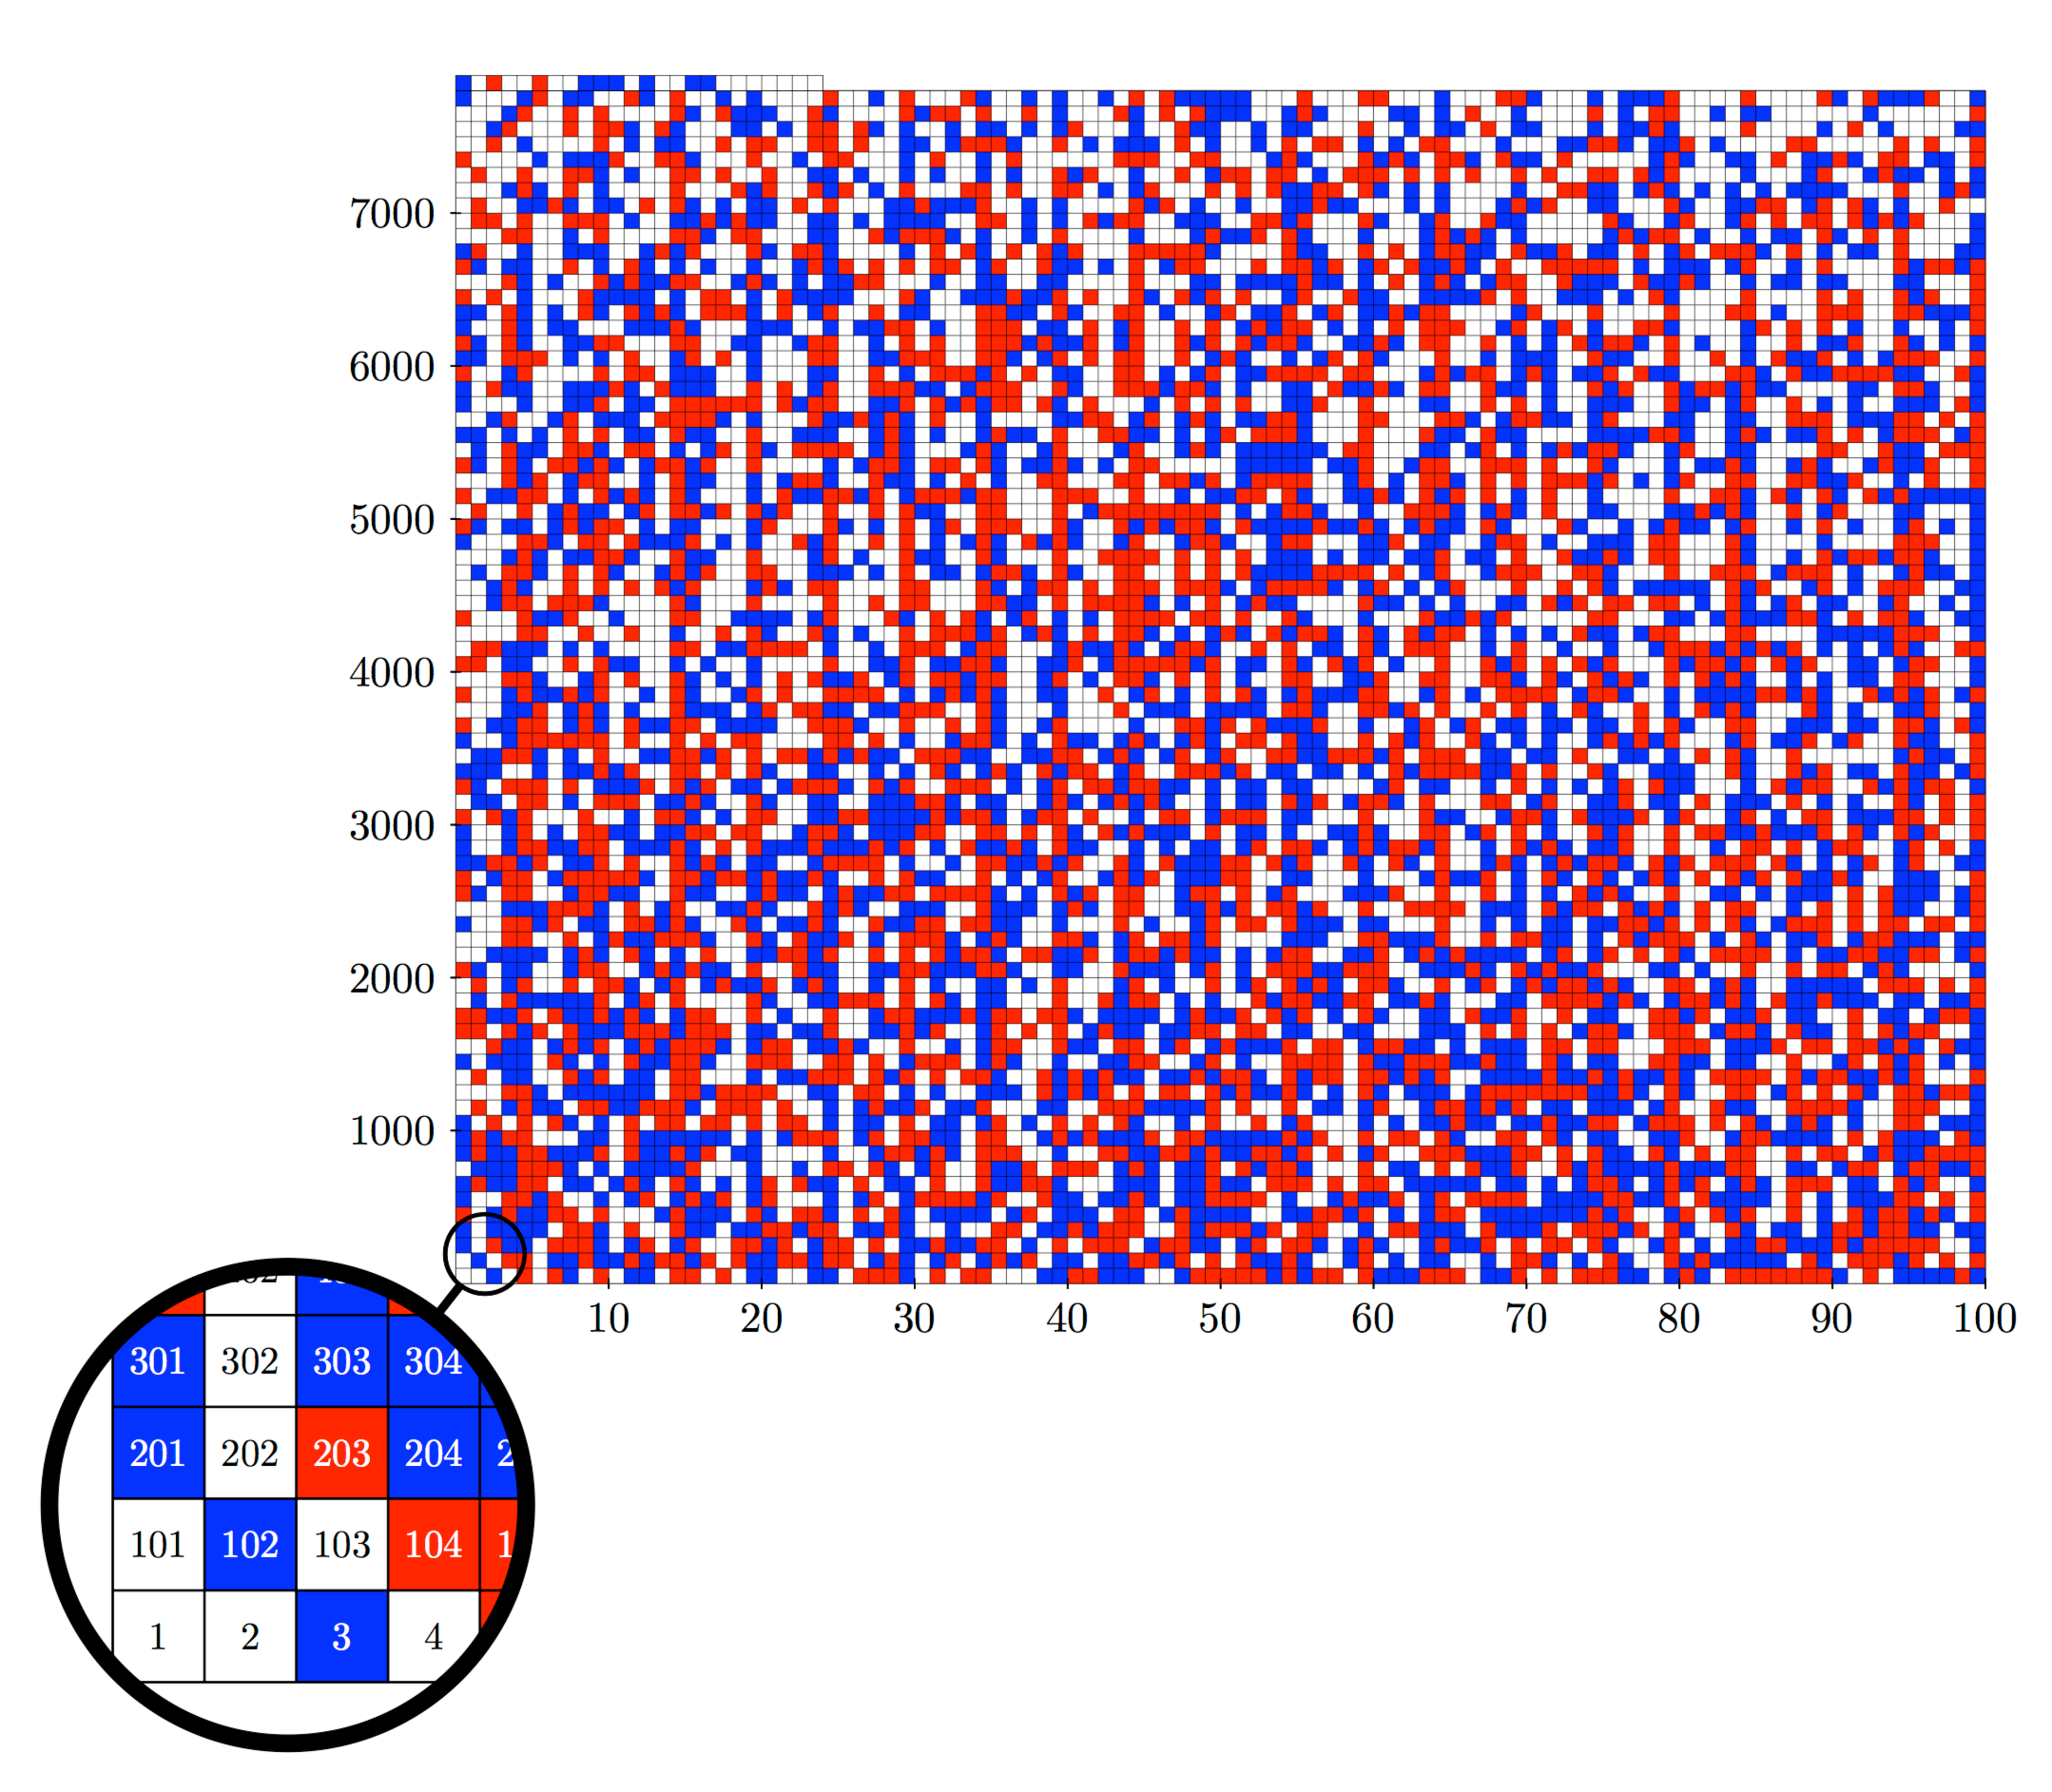
\includegraphics[height=3in]{figs/triple7824}
\end{center}

\end{frame}

\begin{frame}
\frametitle{SAT Application: Coloring Pythagorean Triples, $n\geq 7825$}

{\bf Formula ${\it PTC}(7825)$ unsatisfiable}
\begin{itemize}
\item Heule, Kullmann, Marek, SAT 2016

\medskip

\item Partitioned into $10^6$ subproblems
  \begin{itemize}
    \item By enumerating assignments for some of the variables
  \end{itemize}

\medskip

  
\item Ran on 800-core supercomputer for two days

\medskip

\item Generated $10^6$ proofs of unsatisfiability
  \begin{itemize}
  \item 200 Terabytes total
  \item Validated with proof checker
  \item A very long and very tedious collection of proofs!
  \end{itemize}

\item Unsatisfiability proof provides mathematical rigor
\end{itemize}

\end{frame}

\frame{
\frametitle{Boolean Satisfiability Solvers}


\begin{tikzpicture}


\node[text width=1.5cm] (F) at (0,0) {Boolean formula};
\node[regular polygon,regular polygon sides=4, minimum size=3.5cm, draw,fill=structure, rounded corners] (S) at (3.5,0) {};
\node[white] at (3.5,0.5) {\huge \bf SAT};
\node[white] at (3.5,-0.5) {\huge \bf solver};
\draw[line width=3pt, -latex] (F) -- (S);
\node[white] at (10,3.75) {~};

\node[text width=1.5cm] (sat) at (8,0.75) {\large \bf solution};
\node (topl) at (4.75,0.75) {~};
\draw[line width=2pt, -latex] (topl) -- (sat);
\node  at (6,1.25) {{\it satisfiable}};


\node[text width=1.5cm] (unsat) at (8,-0.75) {\large \bf ?};
\node  at (6,-0.25) {{\it unsatisfiable}};
\node (botl) at (4.75,-0.75) {~};
\draw[line width=2pt, -latex] (botl) --(unsat);

\node[rectangle, minimum height=1.5cm,minimum width=3cm, draw,fill=xgreen, rounded corners] (check) at (8.5,3) {};
\node[white] at (8.5,3.25) {\large \bf Solution};
\node[white] at (8.5,2.75) {\large \bf Checker};

\draw[line width=3pt, -latex] (F) edge [bend left=20] (check.west);
\draw[line width=2pt, -latex] (sat.north) -- (check.south);


\end{tikzpicture}

\bigskip

\begin{minipage}{.40\textwidth}
{\bf SAT Solvers Useful}
\begin{itemize}
\item Optimization
\item Formal verification
\item Mathematical proofs
\end{itemize}
\end{minipage}
\begin{minipage}{.58\textwidth}
{\bf Can We Trust Them?}
\begin{itemize}
\item No!
\item Complex software
\item e.g., KISSAT: 35K lines of code
\end{itemize}
\end{minipage}



}


\frame{
\frametitle{Proof Generating Solvers}

\begin{tikzpicture}


\node[text width=1.5cm] (F) at (0,0) {Boolean formula};

\node[regular polygon,regular polygon sides=4, minimum size=3.5cm, draw,fill=structure, rounded corners] (S) at (3.5,0) {};
\node[white] at (3.5,0.5) {\huge \bf SAT};
\node[white] at (3.5,-0.5) {\huge \bf solver};
\node[white] at (10,3.75) {~};
\draw[line width=3pt, -latex] (F) --( S);

\node[text width=1.5cm] (unsat) at (8,-0.75) {\large \bf unsatisfiability proof};
\node  at (6,-0.25) {{\it unsatisfiable}};
\node (botl) at (4.75,-0.75) {~};
\draw[line width=2pt, -latex] (botl) --(unsat);

\node[rectangle, minimum height=1.5cm,minimum width=3cm, draw,fill=xgreen, rounded corners] (check) at (8.5,3) {};
\node[white] at (8.5,3.25) {\large \bf Proof};
\node[white] at (8.5,2.75) {\large \bf Checker};

\draw[line width=3pt, -latex] (F) edge [bend left=20] (check.west);
\draw[line width=2pt, -latex] (unsat.north) -- (check.south);

\end{tikzpicture}

\bigskip
\bigskip

\begin{minipage}{.49\textwidth}
{\bf Unsatisfiability Proof}
\begin{itemize}
\item Step-by-step proof in\\some logical framework
\end{itemize}
\end{minipage}
\begin{minipage}{.49\textwidth}
{\bf Proof Checker}
\begin{itemize}
\item Simple program
\item May be formally verified
\end{itemize}
\end{minipage}

} %% FRAME


\frame{
  \frametitle{Impact of Proof Checking}

  \begin{minipage}[t]{0.43\textwidth}
    {\bf Adoption}
    \begin{itemize}
      \item Required for SAT competition entrants since 2016
    \end{itemize}
    {\bf Benefits}
    \begin{itemize}
    \item Can clearly judge competition submissions
    \item Developers have improved quality of their solvers
    \item Firm foundation for use in mathematical proofs
    \end{itemize}
  \end{minipage}
  \begin{minipage}[t]{0.03\textwidth}
    $\;$
  \end{minipage}  
  \begin{minipage}[t]{0.50\textwidth}
    {\bf Unintended Consequences}
    \begin{itemize}
    \item Narrowed focus to single SAT algorithm
      \begin{itemize}
      \item Conflict-Driven Clause Learning (CDCL)
      \item Search for solution, but learn conflicts
      \end{itemize}
    \item Other powerful solution methods have languished.
    \end{itemize}
    \only <2>{
    {\bf My Long-Term Goals}
    \begin{itemize}
    \item Enable proof generation for other SAT algorithms
    \item Develop checkable proof infrastructure for other domains
    \end{itemize}
    }
  \end{minipage}
}


\frame{
\frametitle{Conjunctive Normal Form (CNF) Formulas}

{\bf Variables}
\begin{itemize}
\item Input: $X = \{x_1, x_2, \ldots, x_n\}$
\item Informally: $a, b, c, \ldots$
\end{itemize}

{\bf Literals}
\begin{itemize}
\item Variable $x$
\item Complemented variable $\xnot$.
\end{itemize}

{\bf Clauses}
\begin{itemize}
\item \makebox[1.5in][l]{$C = \{\ell_1, \ell_2, \ldots, \ell_k\}$}Set of literals
\item $\anot \lor b \lor \cnot$
\item \makebox[1.5in][l]{$\bot = \emptyset$}Empty clause (False)
\end{itemize}

{\bf Formula}
\begin{itemize}
\item $\phi = \{ C_1,  C_2, \ldots, C_m \}$
\item \makebox[1.5in][l]{$C_1 \land  C_2 \land \cdots \land C_m$}Conjunction of clauses
\end{itemize}
}

\frame{
\frametitle{Clausal Thinking}

{\bf Useful tricks when writing CNF}

\begin{center}
  \renewcommand{\arraystretch}{1.2}
  \begin{tabular}{cc}
    \toprule
    \makebox[1.5in]{Boolean Formula} & \makebox[1.5in]{CNF} \\
    \midrule
    $a \land b \rightarrow c$ & $\anot \lor \bnot \lor c$ \\
    $a \rightarrow b \lor c$ & $\anot \lor b \lor c$ \\
    $(a \lor b) \rightarrow c$ & $(\anot \lor c) \land (\bnot \lor c)$ \\
    $a \rightarrow (b \land c)$ & $(\anot \lor b) \land (\anot \lor c)$ \\
    $\ite(a, b, c)$ & $(\anot \lor b) \land (a \lor c)$ \\
    \bottomrule
  \end{tabular}
\end{center}

\begin{itemize}
\item Advice: think in terms of implication.
\item E.g., $\ite(a, b, c) =  (a\rightarrow b) \land (\obar{a} \rightarrow c)$
\end{itemize}


}

\frame{
\frametitle{Clausal Thinking: Parity Encodings}

\begin{center}
  \renewcommand{\arraystretch}{1.2}
  \begin{tabular}{ccl}
    \toprule
    \makebox[1.5in]{Boolean Formula} & \makebox[1.5in]{CNF} & \makebox[1in]{Explanation}\\
    \midrule
    ${\it OddParity}(a, b, c)$ &
    $\begin{array}{ll}
      (\anot \lor \bnot \lor c) & \land\\
      (\anot \lor b \lor \cnot) & \land\\
      (a \lor \bnot \lor \cnot) & \land\\
      (a \lor b \lor c) & \\
    \end{array}$ 
    &
    \begin{tabular}{l}
      Even number  \\of negations
    \end{tabular}

    \\
\midrule
    ${\it EvenParity}(a, b, c)$ &
    $\begin{array}{ll}
      (\anot \lor \bnot \lor \cnot) & \land\\
      (a \lor b \lor \cnot) & \land\\
      (a \lor \bnot \lor c) & \land \\
      (\anot \lor b \lor c) & \\
    \end{array}$ 
    &
    \begin{tabular}{l}
      Odd number  \\of negations
    \end{tabular}
    \\
    \bottomrule
  \end{tabular}
\end{center}
}

\frame{
\frametitle{Clausal Thinking: Parity Encodings}

\begin{center}
  \renewcommand{\arraystretch}{1.05}
  \begin{tabular}{cc}
    \toprule
    \makebox[2in]{Boolean Formula} & \makebox[2in]{CNF} \\
    \midrule
    ${\it OddParity}(a, b, c)$ &
    $\begin{array}{ll}
      (\anot \lor \bnot \lor c) & \land\\
      (\anot \lor b \lor \cnot) & \land\\
      (a \lor \bnot \lor \cnot) & \land\\
      (a \lor b \lor c) & \\
    \end{array}$ \\
\midrule
    ${\it OddParity}(a, b, c, d)$ &
    $\begin{array}{ll}
      (\anot \lor \bnot \lor \cnot \lor \dnot) & \land\\
      (a \lor b \lor \cnot \lor \dnot) & \land\\
      (a \lor \bnot \lor c \lor \dnot) & \land \\
      (\anot \lor b \lor c \lor \dnot) & \land\\
      (\anot \lor \bnot \lor c \lor d) & \land\\
      (\anot \lor b \lor \cnot \lor d) & \land\\
      (a \lor \bnot \lor \cnot \lor d) & \land\\
      (a \lor b \lor c \lor d) & \\
    \end{array}$ \\
    \bottomrule
  \end{tabular}
\end{center}
}

\frame{
  \frametitle{Parity Encoding with Intermediate Variables}
{\bf Task}
 \begin{itemize}
 \item Encode ${\it OddParity}(x_1, x_2, \ldots, x_n)$
 \item Direct encoding requires  $2^{n-1}$ clauses
 \item All combinations with even number of negative literals
 \end{itemize}

{\bf Decomposition}
     \begin{itemize}
     \item Introduce new variable $z$
     \item Directly encode ${\it EvenParity}(x_1, x_2, z)$
     \item Recursively encode ${\it OddParity}(z, x_3, x_4, \ldots, x_n)$:
       \begin{itemize}
       \item If $x_1 \oplus x_2 = 0$, then $z = 0$ and ${\it OddParity}(x_3, x_4, \ldots, x_n)$
       \item If $x_1 \oplus x_2 = 1$, then $z = 1$ and ${\it EvenParity}(x_3, x_4, \ldots, x_n)$         
       \end{itemize}
     \end{itemize}

} %% Frame

\frame{
  \frametitle{Parity Encoding with Intermediate Variables}
{\bf Decomposition}
     \begin{itemize}
     \item Directly encode ${\it EvenParity}(x_1, x_2, z)$
     \item Recursively encode ${\it OddParity}(z, x_3, x_4, \ldots, x_n)$:
     \end{itemize}
\medskip
{\bf General Form}
\begin{eqnarray*}
  z_2 &=& x_1 \oplus x_2 \\
  z_3 &=& z_2 \oplus x_3 \\
  & \cdots & \\
  z_{n-2} & = & x_{n-2} \oplus x_{n-3}\\
  z_{n-2} \oplus x_{n-1} \oplus x_n & = & 1\\
\end{eqnarray*}
\vskip -15pt
{\bf Complexity}
\begin{itemize}
\item $n-3$ additional variables
\item $4(n-2)$ clauses
\end{itemize}
} %% Frame

\frame{
\frametitle{Clausal Thinking: Cardinality Constraints}

\begin{eqnarray*}
a_1 \, x_1 + a_2 \, x_2 + \cdots + a_n \, x_n & \geq & t
\end{eqnarray*}


\begin{center}
  \renewcommand{\arraystretch}{1.1}
\begin{tabular}{rcc}
  \makebox[1in]{Constraint} & \makebox[.5in]{$a_i$} & \makebox[.5in]{$t$} \\
\midrule
 ${\it AtLeastOne}$ &  $\{0, 1\}$ &  $1$ \\
 ${\it AtMostOne}$  &  $\{0, -1\}$ & $-1$ \\
\end{tabular}

\end{center}

\begin{center}
  \renewcommand{\arraystretch}{1.2}
  \begin{tabular}{cc}
    \toprule
    \makebox[2in]{Boolean Formula} & \makebox[2in]{CNF} \\
    \midrule
    ${\it AtLeastOne}(a, b, c)$ & $a \lor b \lor c$ \\
    ${\it AtMostOne}(a, b, c)$ & $(\anot \lor \bnot) \land (\anot \lor \cnot) \land (\bnot \lor \cnot)$ \\
    ${\it AtMostOne}(a, b, c, d)$ &
    $\begin{array}{ll}
      (\anot \lor \bnot) \land (\anot \lor \cnot) \land (\anot \lor \dnot) & \land \\
      (\bnot \lor \cnot) \land (\bnot \lor \dnot) \land (\cnot \lor \dnot) & \\
    \end{array}$ \\
    \bottomrule
  \end{tabular}
\end{center}


}


\frame{
\frametitle{Encoding Arbitrary Formulas / Circuits}

\begin{center}
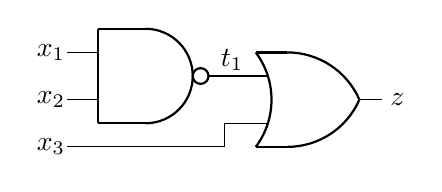
\begin{tikzpicture}[scale=0.20]
  %% NAND gate
   \draw [thick] (2,7.5) -- (5,7.5);
   \draw [thick] (2,1.5) -- (5,1.5);
   \draw [thick] (2,7.5) -- (2,1.5);
   \draw [thick] (5,1.5) arc [radius=3, start angle = -90, end angle = 90];
   \draw [thick] (8.5,4.5) circle [radius=0.5];
   %% OR gate
   \draw [thick] (12,6) -- (14,6);
   \draw [thick] (12,0) -- (14,0);
   \draw [thick] (12,6) arc [radius=5, start angle = 36.9, end angle = -36.9];
   \draw [thick] (14, 6) arc [radius=5, start angle = 90, end angle = 23.6];
   \draw [thick] (14, 0)  arc [radius=5, start angle = -90, end angle = -23.6];
   \draw (18.6,3) -- (20,3);
  %% Wire it up
  \draw (0,6) -- (2,6);
  \draw (0,3) -- (2,3);
  \draw (0,0) -- (10,0) -- (10,1.5) -- (12.8,1.5);
  \draw (9,4.5) -- (12.8,4.5);
  %% Put in labels
  \node at (-1,6) {$x_1$};
  \node at (-1,3) {$x_2$};
  \node at (-1,0) {$x_3$};
  \node at (10.5,5.5) {$t_1$};
  \node at (21,3) {$z$};
\end{tikzpicture}
\end{center}
\renewcommand{\arraystretch}{1.1}
\begin{tabular}{lcc}
  \toprule
  \makebox[0.5in]{} & \makebox[1.75in]{Encode NAND gate} & \makebox[1.75in]{Encode OR gate} \\
  \midrule
  Formula
     & $\tnot_1 \leftrightarrow x_1 \land x_2$  
     & $z \leftrightarrow t_1 \lor x_3$  \\
  \midrule
  Clauses 
     &  $\begin{array}{l}
        t_1 \lor x_1 \\
       t_1 \lor x_2 \\
        \tnot_1 \lor \xnot_1 \lor \xnot_2\\
       \end{array}$
     &  $\begin{array}{l}
        \znot \lor t_1 \lor x_3 \\
        z \lor \tnot_1 \\
        z \lor \xnot_3 \\
       \end{array}$ \\
  \bottomrule
\end{tabular}

\medskip

    {\bf Tseitin Encoding}
    \begin{itemize}
    \item Introduce variables for intermediate values
    \item Linear complexity
    \end{itemize}


} %% FRAME

\frame{
  \frametitle{Proof Rules: Resolution}

\begin{itemize}
\item Robinson, 1965
\end{itemize}

\begin{center}
\begin{tikzpicture}
\node at (2.5,0) {$\anot \lor b \lor \structure{x}$};
\node at (5,0) {$\structure{\xnot} \lor c \lor \dnot$};
\draw[thick] (1.5,-0.25) -- (6.2,-0.25);
\node at (3.75,-0.5) {$(\anot \lor b) \lor (c \lor \dnot)$};
\only<2->{
\node at (1,1) {$(a \land \bnot) \rightarrow \structure{x}$};
\node at (6.5,1) {$\structure{x} \rightarrow (c \lor \dnot)$};
\node at (3.75,-1.5) {$(a \land \bnot) \rightarrow (c \lor \dnot)$};
}
\end{tikzpicture}
\end{center}
\begin{itemize}
\item Generalization of implication
\item See  \hcref{https://en.wikipedia.org/wiki/Resolution\_(logic)}
\end{itemize}  


} %% FRAME

\frame{
  \frametitle{Resolution Principle Nuances}


\bigskip

{\bf OK To Have Repeated Literal}

\medskip

\begin{center}
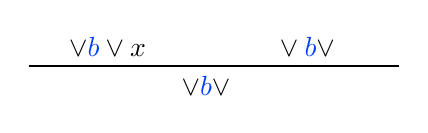
\begin{tikzpicture}
\node at (2.5,0) {$\anot \lor \textcolor{xblue}{b} \lor \structure{x}$};
\node at (5,0) {$\structure{\xnot} \lor \textcolor{xblue}{b} \lor \dnot$};
\draw[thick] (1.5,-0.25) -- (6.2,-0.25);
\node at (3.75,-0.5) {$\anot \lor \textcolor{xblue}{b} \lor \dnot$};
\end{tikzpicture}
\end{center}

\medskip

{\bf Not OK to Have Multiple Resolution Variables}

\medskip

\begin{center}
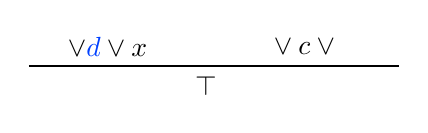
\begin{tikzpicture}
\node at (2.5,0) {$\anot \lor \textcolor{xblue}{d} \lor \structure{x}$};
\node at (5,0) {$\structure{\xnot} \lor c \lor \textcolor{xblue}{\dnot}$};
\draw[thick] (1.5,-0.25) -- (6.2,-0.25);
\node at (3.75,-0.5) {$\top$};
\end{tikzpicture}
\end{center}


} %% FRAME

\frame{
  \frametitle{Proof Rules: Subsumption}

  \bigskip
  
\begin{center}
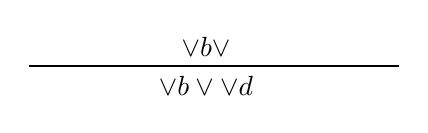
\begin{tikzpicture}
\node at (3.75,0) {$\anot \lor b \lor \cnot$};
\draw[thick] (1.5,-0.25) -- (6.2,-0.25);
\node at (3.75,-0.5) {$\anot \lor b \lor \cnot \lor \structure{d}$};
\end{tikzpicture}
\end{center}
\begin{itemize}
\item General Principle: $F \rightarrow F \lor d$
\end{itemize}  


} %% FRAME




\frame{
  \frametitle{Example Formula}

  {\bf DIMACS Format}
  \begin{itemize}
    \item Standard for all solvers
    \item Positive integers for variables
    \item Negative integers for their negations
    \item Lists terminated with {\tt 0}
  \end{itemize}  

  \begin{center}
    \begin{tabular}{cll}
      \toprule
      \makebox[0.5in]{ID} & \makebox[1.0in]{Clause} & \makebox[1.5in]{DIMACS Encoding} \\
      \midrule
      & & {\tt p cnf 4 6} \\
      1 & $\anot \lor \bnot \lor \cnot$ & {\tt -1 -2 -3 0} \\
      2 & $\anot \lor \bnot \lor c$ & {\tt -1 -2  3 0} \\
      3 & $a \lor \dnot$ & {\tt 1    -4 0} \\
      4 & $a \lor d$ & {\tt 1    4 0} \\
      5 & $b \lor \dnot$ & {\tt    2     -4 0} \\
      6 & $b \lor d$ & {\tt    2     4 0} \\
      \bottomrule
    \end{tabular}
  \end{center}
}

\frame{
  \frametitle{Example Proof}

\begin{itemize}
\item Derive empty clause $\bot$ through set of resolution steps
\end{itemize}

\begin{center}
\begin{tikzpicture}[scale = 0.8]
\node at (5.5,4.0) {$a \lor d$};
\node at (7.5,4.0) {$a \lor \dnot$};
\draw[thick] (4.5,3.5) -- (8.5,3.5);
\node at (5.0,3.0) {$a$};
\node at (8.0,3.0) {$a$};

\node at (3.0,3.0) {$\anot \lor \bnot \lor c$};
\draw[thick] (2.0,2.5) -- (5.5,2.5);
\node at (4.0,2.0) {$\bnot \lor c$};

\node at (10.0,3.0) {$\anot \lor \bnot \lor \cnot$};
\draw[thick] (7.5,2.5) -- (11.0,2.5);
\node at (9.0,2.0) {$\bnot \lor \cnot$};
\draw[thick] (3.5,1.5) -- (9.5,1.5);
\node at (6.5,1.0) {$\bnot$};

\node at (12.0,2.0) {$b \lor \dnot$};
\node at (14.0,2.0) {$b \lor d$};
\draw[thick] (11.5,1.5) -- (14.5,1.5);
\node at (13.0,1.0) {$b$};
\draw[thick] (6.0,0.5) -- (13.5,0.5);
\node at (9.750,0.0) {$\bot$};
\end{tikzpicture}

\end{center}

{\em \textcolor{xblue}{But how can a program find such a proof?}}


} %% FRAME




\begin{frame}
\frametitle{Unit Propagation}

{\bf Unit clauses}
\begin{itemize}
  \item If formula contains clause $(x)$, then $x$ must be assigned $1$.
  \item If formula contains clause $(\obar{x})$, then $x$ must be assigned $0$.
\end{itemize}
{\bf Propagating Unit Literal $\ell$}
\begin{itemize}
\item If $\ell \in C$ and $\ell=0$, then $C \leftarrow C-\{\ell\}$
\item If $\ell \in C$ and $\ell=1$, then $C$ satisfied
\item If any clause becomes unit, then iterate
\end{itemize}

\centering{
  \renewcommand{\arraystretch}{1.2}
  \begin{tabular}{ccc}
    \toprule
    \makebox[.5in]{Step} & \makebox[3in]{Formula} & \makebox[.5in]{Units} \\
    \midrule
    1 & $\bm{(a \lor \cnot) \land (\anot \lor \bnot \lor \cnot) \land (a \lor b \lor c) \land (c)}$ & $c = 1$ \\
    2 & $\bm{(a \lor \gtext{\cnot}) \land (\anot \lor \bnot \lor \gtext{\cnot}) \land (a \lor b \lor \rtext{c}) \land (\rtext{c})}$ & $a = 1$ \\
    3 & $\bm{(\rtext{a} \lor \gtext{\cnot}) \land (\gtext{\anot} \lor \bnot \lor \gtext{\cnot}) \land (\rtext{a} \lor b \lor \rtext{c}) \land (\rtext{c})}$ & $b = 0$ \\
    -- & $\bm{(\rtext{a} \lor \gtext{\cnot}) \land (\gtext{\anot} \lor \rtext{\bnot} \lor \gtext{\cnot}) \land (\rtext{a} \lor \gtext{b} \lor \rtext{c}) \land (\rtext{c})}$ &  \\
    \bottomrule
  \end{tabular}
} % Centering
\end{frame}

\begin{frame}
  \frametitle{Basic CDCL Operation}

  {\bf Conflict-Driven Clause Learning}
  \begin{itemize}
    \item Algorithm in state-of-the art solvers
    \item Search, but learn from dead ends
  \end{itemize}

\begin{tabbing}
xxxxxx\=xxxx\=xxxx\=xxxx\=\kill
\>\keywhile(\keytrue): \\
\>\>${\it depth}\; \assign \;0$ \\
\>\>\keywhile(\keytrue): \\
\>\>\>UnitPropagate() \\
\>\>\>\keyif{} all clauses satisfied \\
\>\>\>\>\keyreturn{} solution\\
\>\>\>\keyif{} ConflictDetected(): \\
\>\>\>\>Generate conflict clause \\
\>\>\>\>\keybreak{} \\
\>\>\>Choose variable and assign $0$ or $1$\\
\>\>\>${\it depth} \;\assign \; {\it depth} + 1$ \\
\>\>\keyif{} ${\it depth} = 0$: \\
\>\>\>\keyreturn{} UNSAT\\
\end{tabbing}


\end{frame}

\begin{frame}
\frametitle{CDCL Execution Example}
\begin{itemize}
\item
  \only<1>{No initial unit propagations}
  \only<2>{Setting $b=0$ causes conflict.  Learn clause $b$.}
  \only<3>{Unit propagate $b$.  No conflict}
  \only<4>{Setting $c=1$ causes conflict.  Learn clause $\cnot$.}  
  \only<5>{Unit propagate $b$ and $\cnot$.  Causes conflict.  UNSAT!}
\end{itemize}
\medskip
\begin{minipage}{0.4\textwidth}
\input{cdcl-dd/cdcl}
\end{minipage}
\begin{minipage}[t]{0.57\textwidth}
  \renewcommand{\arraystretch}{1.1}
    \begin{tabular}{clc}
      \toprule
      \makebox[0.5in]{ID} & \makebox[0.75in][l]{Clause} & \makebox[0.5in][c]{UProp?} \\
      \midrule
      1 & ${\anot \lor \bnot \lor \cnot}$ & \only<4>{*}  \\
      2 & ${\anot \lor \bnot \lor c}$     & \only<5>{*} \\
      3 & ${a \lor \dnot}$                & \only<4-5>{*} \\
      4 & ${a \lor d}$                    & \only<4-5>{*} \\
      5 & ${b \lor \dnot}$                & \only<2>{*} \\
      6 & ${b \lor d}$                    &  \only<2>{*} \\
      \bottomrule
  \only<2->{7} & \only<2->{${b}$}        & \only<4-5>{*} \\
  \only<4->{8} & \only<4->{${\cnot}$}    & \only<5>{*} \\
  \only<5->{9} & \only<5->{${\bot}$}     & \\
    \end{tabular}
\end{minipage}
\end{frame}

\frame{
  \frametitle{Proof from CDCL Run}

{\bf Proof Follows Branching Structure of CDCL}

\medskip

\begin{minipage}{0.98\textwidth}
\begin{minipage}{0.3\textwidth}
\input{cdcl-dd/cdcl-flip}
\end{minipage}
\begin{minipage}{0.65\textwidth}
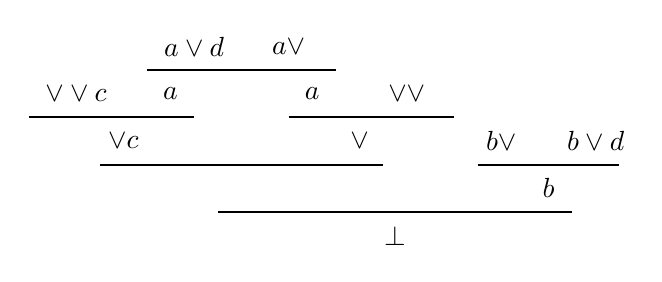
\begin{tikzpicture}[scale = 0.6]
\node at (5.5,4.0) {$a \lor d$};
\node at (7.5,4.0) {$a \lor \dnot$};
\draw[thick] (4.5,3.5) -- (8.5,3.5);
\node at (5.0,3.0) {$a$};
\node at (8.0,3.0) {$a$};

\node at (3.0,3.0) {$\anot \lor \bnot \lor c$};
\draw[thick] (2.0,2.5) -- (5.5,2.5);
\node at (4.0,2.0) {$\bnot \lor c$};

\node at (10.0,3.0) {$\anot \lor \bnot \lor \cnot$};
\draw[thick] (7.5,2.5) -- (11.0,2.5);
\node at (9.0,2.0) {$\bnot \lor \cnot$};
\draw[thick] (3.5,1.5) -- (9.5,1.5);
\node at (6.5,1.0) {$\bnot$};

\node at (12.0,2.0) {$b \lor \dnot$};
\node at (14.0,2.0) {$b \lor d$};
\draw[thick] (11.5,1.5) -- (14.5,1.5);
\node at (13.0,1.0) {$b$};
\draw[thick] (6.0,0.5) -- (13.5,0.5);
\node at (9.750,0.0) {$\bot$};
\end{tikzpicture}
\end{minipage}
\end{minipage}


} %% FRAME

\begin{frame}
  \frametitle{Reverse Unit Propagation (RUP)}

  {\bf Purpose}
  \begin{itemize}
  \item Simple and efficient rule for use by proof checkers
  \item Good match to operation of CDCL solvers
  \end{itemize}

  {\bf Operation}
  \begin{itemize}
  \item Each RUP application forms one step of unsatisfiability proof
  \item Performs a linear sequence of resolutions steps + subsumption
  \end{itemize}

  {\bf Objective}
  \begin{itemize}
    \item \makebox[1.35in][l]{$C = \{\ell_1, \ell_2, \ldots, \ell_m\}$} Clause to be added to proof
    \item \makebox[1.35in][l]{$D_1, D_2, \ldots, D_k$} Previous clauses (``Antecedents'')
    \item Prove: $D_1 \land D_2 \land \cdots \land D_k \rightarrow C$ 
  \end{itemize}

\end{frame}


\begin{frame}
  \frametitle{Reverse Unit Propagation (RUP)}

  {\bf Objective}
  \begin{itemize}
    \item \makebox[1.35in][l]{$C = \{\ell_1, \ell_2, \ldots, \ell_m\}$} Clause to be added to proof
    \item \makebox[1.35in][l]{$D_1, D_2, \ldots, D_k$} Previous clauses (``Antecedents'')
    \item Prove: $D_1 \land D_2 \land \cdots \land D_k \rightarrow C$ 
  \end{itemize}
{\bf Method}
\begin{itemize}
\item Assume $\neg C = \obar{\ell}_1 \land \obar{\ell}_2 \land \cdots \land \obar{\ell}_m$
  \begin{itemize}
    \item $m$ unit clauses!
  \end{itemize}
\item Show contradiction with $D_1 \land D_2 \land \cdots \land D_k$ 
  \begin{itemize}
  \item Accumulate unit clauses, starting with those for $\neg C$.
  \item Accrue more unit clauses from $D_1, D_2, \ldots, D_{k-1}$.
  \item When encounter $D_k$, should have contradiction
  \end{itemize}
\end{itemize}

\end{frame}

\begin{frame}
\frametitle{RUP Proof Example}
\centering{
  \renewcommand{\arraystretch}{1.1}
    \begin{tabular}{cll}
      \toprule
      \makebox[0.5in]{ID} & \makebox[0.75in][l]{Clause} & \makebox[1in][c]{Antecedents} \\
      \midrule
      $C_1$ & ${\anot \lor \bnot \lor \cnot}$ & \\
      $C_2$ & ${\anot \lor \bnot \lor c}$     & \\
      $C_3$ & ${a \lor \dnot}$                & \\
      $C_4$ & ${a \lor d}$                    & \\
      $C_5$ & ${b \lor \dnot}$                & \\
      $C_6$ & ${b \lor d}$                    & \\
      \bottomrule
  \only<2->{$C_7$} & \only<2->{${b}$}        & \only<2->{$C_5, C_6$} \\
  \only<3->{$C_8$} & \only<3->{${\cnot}$}    & \only<3->{$C_7, C_1, C_3, C_4$} \\
  \only<4->{$C_9$} & \only<4->{${\bot}$}     & \only<4->{$C_7, C_8, C_2, C_3, C_4$} \\
    \end{tabular}
}
\vskip -10pt
\only<2>{
\begin{tabular}{c|ccccccccccc}
  \multicolumn{1}{c}{\makebox[0.2in]{}} &
  \makebox[0.10in]{} &   \makebox[0.10in]{} &  \makebox[0.10in]{} &  \makebox[0.10in]{}
  &  \makebox[0.10in]{} &  \makebox[0.10in]{} &  \makebox[0.10in]{} &  \makebox[0.10in]{} &  \makebox[0.10in]{} &  \makebox[0.10in]{} &  \makebox[0.10in]{} \\
          & \rtext{$\bnot$} &        & \rtext{$\dnot$} &       & \rtext{$\bot$} \\
      $b$ &         & $C_5$  &         & $C_6$ &  \\
\end{tabular}
}
\only<3>{
\begin{tabular}{c|ccccccccccc}
  \multicolumn{1}{c}{\makebox[0.2in]{}} &
  \makebox[0.10in]{} &   \makebox[0.10in]{} &  \makebox[0.10in]{} &  \makebox[0.10in]{}
  &  \makebox[0.10in]{} &  \makebox[0.10in]{} &  \makebox[0.10in]{} &  \makebox[0.10in]{} &  \makebox[0.10in]{} &  \makebox[0.10in]{} &  \makebox[0.10in]{} \\
              &     \rtext{$c$} &        & \rtext{$b$}     &       & \rtext{$\anot$} &       & \rtext{$\dnot$} &        & \rtext{$\bot$} \\
      $\cnot$ &         & $C_7$  &         & $C_1$ &         & $C_3$ &         & $C_4$ \\
\end{tabular}
}
\only<4>{
\begin{tabular}{c|ccccccccccc}
  \multicolumn{1}{c}{\makebox[0.2in]{}} &
  \makebox[0.10in]{} &   \makebox[0.10in]{} &  \makebox[0.10in]{} &  \makebox[0.10in]{}
  &  \makebox[0.10in]{} &  \makebox[0.10in]{} &  \makebox[0.10in]{} &  \makebox[0.10in]{} &  \makebox[0.10in]{} &  \makebox[0.10in]{} &  \makebox[0.10in]{} \\
              &         &        & \rtext{$b$}     &       & \rtext{$\cnot$} &       & \rtext{$\anot$} &        & \rtext{$\dnot$} &    & \rtext{$\bot$} \\
      $\bot$  &         & $C_7$  &         & $C_8$ &         & $C_2$ &         & $C_3$   &         & $C_4$      \\
\end{tabular}
}
\end{frame}

\begin{frame}
\frametitle{Proof File Examples}

\centering{
   \begin{tabular}{cll}
   \multicolumn{3}{l}{Proof} \\
  \midrule
  \makebox[0.5in][c]{$C_7$} & \makebox[0.75in][l]{${b}$}        & \makebox[1in][l]{$C_5, C_6$} \\
  {$C_8$} & {${\cnot}$}    & {$C_7, C_1, C_3, C_4$} \\
  {$C_9$} & {${\bot}$}     & {$C_7, C_8, C_2, C_3, C_4$} \\
  \bottomrule
  &&\\
  \multicolumn{3}{l}{DRAT Proof File} \\
  \toprule 
          & {\tt 2 0} & \\
          & {\tt -3 0} & \\
          & {\tt 0} & \\
  \bottomrule
  && \\
  \multicolumn{3}{l}{LRAT Proof File} \\
  \toprule 
     {\tt 7}     & {\tt 2 0} & {\tt 5 6 0}\\
     {\tt 8}     & {\tt -3 0} & {\tt 7 1 3 4 0}\\
     {\tt 9}     & {\tt 0} &   {\tt 7 8 2 3 4 0}\\
  \bottomrule 
  \end{tabular}
}
\end{frame}


\begin{frame}
  \frametitle{Proof Checking Infrastructure}

  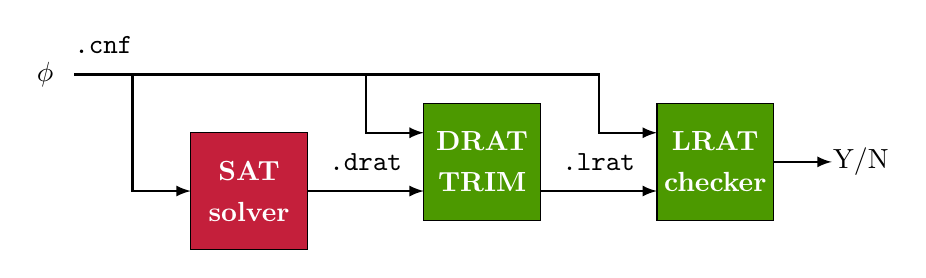
\begin{tikzpicture}[scale=0.37]
  \draw[fill=xred] (5,3) rectangle (9,7);
  \node[white] at (7,5.7) {\bf SAT};
  \node[white] at (7,4.3) {\bf solver};
  \draw[fill=xgreen] (13,4) rectangle (17,8);
  \node[white] at (15,6.7) {\bf DRAT};
  \node[white] at (15,5.3) {\bf TRIM};
  \draw[fill=xgreen] (21,4) rectangle (25,8);
  \node[white] at (23,6.7) {\bf LRAT};
  \node[white] at (23,5.3) {\bf checker};
  \draw[thick,-latex] (1,9) -- (19,9) -- (19,7) -- (21,7);
  \draw[thick,-latex] (11,9) -- (11,7) -- (13,7);
  \draw[thick,-latex] (3,9) -- (3,5) -- (5,5);
  \draw[thick,-latex] (9,5) -- (13,5);
  \draw[thick,-latex] (17,5) -- (21,5);
  \draw[thick,-latex] (25,6) -- (27,6);
  \node at (0,9) {$\phi$};
  \node at (28,6) {Y/N};
  \node at (2,10) {\tt .cnf};
  \node at (11,6) {\tt .drat};
  \node at (19,6) {\tt .lrat};
  \end{tikzpicture}

 {\bf Operation:}
  \begin{itemize}
   \item {\sc Drat-Trim} adds antecedents to proof steps
   \item LRAT checker simply checks each proof step
  \end{itemize}  
{\bf LRAT Checkers:}
\begin{itemize}
\item {\sc lrat-check} written in C.
\begin{itemize}
\item Fast and high capacity
\item Designed to be simple enough to easily understand
\end{itemize}
\item Formally verified ones.  Built on ACL2, Coq, HOL, \ldots
\begin{itemize}
\item Integrity not compromised if solver or {\sc drat-trim} has bug
\end{itemize}
  
\end{itemize}


\end{frame}



\begin{frame}
  \frametitle{Resolution and CDCL}
  
{\bf CDCL $\approx$ Resolution}
\begin{itemize}
\item \makebox[0.75in][l]{{\em Strength:}}CDCL solver can readily generate resolution  proofs 
\item \makebox[0.75in][l]{{\em Weakness:}}Lower bound on performance
\end{itemize}
\medskip

{\bf Example: Pigeonhole Principle(PHP)}
\begin{itemize}
\item Problem:
  \begin{itemize}
    \item $n$ holes, $n+1$ pigeons
    \item Assign pigeons to holes:
      \begin{itemize}
      \item Each pigeon is assigned to some hole
      \item Each hole has at most one pigeon
      \end{itemize}
  \end{itemize}
 \item SAT Encoding:
   \begin{itemize}
     \item Variables: $p_{i,j}$: Pigeon $j$ in hole $i$.  $1 \leq i \leq n$, $1 \leq j \leq n+1$. 
     \item $n+1$ at-least-one constraints
     \item $n$ at-most-one constraints
     \item $O(n^3)$ total clauses
%%     \item For $1 \leq j \leq n+1$: ${\it AtLeastOne}(p_{1,j}, p_{2,j}, \ldots, p_{n,j})$
%%     \item For $1 \leq i \leq n$: ${\it AtMostOne}(p_{i,1}, p_{i,2}, \ldots, p_{i,n+1})$
   \end{itemize}
\item PHP($n$) resolution proofs are exponential in $n$ [Haken, 1985]
\end{itemize}

\end{frame}


\begin{frame}

  \frametitle{Parity Benchmark}

\begin{itemize}
\item Chew and Heule, SAT 2020

\item For random permtuation $\pi$:
\end{itemize}
  \begin{displaymath}
    \begin{array}{cccccccccl}
    x_1 & \oplus & x_2 & \oplus & \cdots & \oplus & x_n & = & 1 & {\sf \;\; Odd \; parity}\\
    x_{\pi(1)} &  \oplus &  x_{\pi(2)} &  \oplus &  \cdots &  \oplus &  x_{\pi(n)} & = & 0& {\sf \;\; Even \; parity}\\
    \end{array}
  \end{displaymath}

  \begin{itemize}
    \item Conjunction unsatisfiable
    \item Very challenging for CDCL solvers
    \item Unit propagation of limited value
      \begin{itemize}
        \item $k$-way parity constraint
        \item Only propagate when $k-1$ variables assigned
      \end{itemize}
  \end{itemize}  

\end{frame}



\begin{frame}
\frametitle{Parity Benchmark Runtime}

\centering{%
\begin{tikzpicture}[scale = .80]
          \begin{axis}[mark options={scale=0.5},grid=both, grid style={black!10}, ymode=log, ymin=0.01, ymax=600.0, xmode=log, legend style={at={(0.95,0.35)}}, legend cell align={left},
                              x post scale=1.6,
                              ytick={0.01,0.1, 1.0, 10.0, 100.0, 600.0}, yticklabels={$0.01$,$0.1$,$1.0$,$10.0$,$100.0$,$600.0$},
                              xtick={10,100,1000,10000,100000}, xticklabels={$10$,$100$,$1{,}000$,$10{,}000$,$100{,}000$},xmin=10,xmax=100000,
            %%                  title={Parity Benchmark Runtime}
            ]
       \input{data-formatted/chew-kissat-seconds}
            \legend{\small \textsf{KISSAT}}
          \end{axis}
\end{tikzpicture}
}

\begin{itemize}
\item KISSAT: State-of-the-art CDCL solver
\item Tried 3-different seeds for each value of $n$
\item Limited to $n \leq 42$ within 600 seconds
\end{itemize}
\end{frame}


\begin{frame}
  \frametitle{Extended Resolution}
  
\begin{itemize}
\item Tseitin, 1967
\end{itemize}

{\bf Can introduce extension variables}
\begin{itemize}
\item Variable $z$ that has not yet occurred in proof
\item Must add {\em defining} clauses
\begin{itemize}
\item Encode constraint of form $z \leftrightarrow F$
\item Boolean formula $z$ over input and earlier extension variables
\end{itemize}
\end{itemize}

\vspace{20pt}

{\bf Extension variable $z$ becomes shorthand for formula $F$}
  \begin{itemize}
  \item Repeated use can yield exponentially smaller proof
  \end{itemize}

  {\bf Similar to use of encoding variables in SAT formulas}
  \begin{itemize}
  \item That's why they're called ``Tseitin variables''
  \item But here they become part of proof, not of input formula
  \end{itemize}

\end{frame}

\begin{frame}
\frametitle{Extended RUP Proof Example}
\begin{center}
  \renewcommand{\arraystretch}{1.1}
    \begin{tabular}{cll}
      \toprule
      \makebox[0.5in]{ID} & \makebox[0.75in][l]{Clause} & \makebox[1in][c]{Antecedents} \\
      \midrule
      $C_1$ & ${\anot \lor \bnot \lor \cnot}$ & \\
      $C_2$ & ${\anot \lor \bnot \lor c}$     & \\
      $C_3$ & ${a \lor \dnot}$                & \\
      $C_4$ & ${a \lor d}$                    & \\
      $C_5$ & ${b \lor \dnot}$                & \\
      $C_6$ & ${b \lor d}$                    & \\
    \bottomrule
    \end{tabular}
\end{center}

    {\bf Strategy}
    \begin{itemize}
    \item Use $z$ to encode $a \land b$.
    \item E.g., $C_1$ becomes $\znot \lor \cnot$.
    \end{itemize}


\end{frame}


\begin{frame}
\frametitle{Extended RUP Proof Example}
\centering{
  \renewcommand{\arraystretch}{1.1}
    \begin{tabular}{cll}
      \toprule
      \makebox[0.5in]{ID} & \makebox[0.75in][l]{Clause} & \makebox[1in][c]{Antecedents} \\
      \midrule
      $C_1$ & ${\anot \lor \bnot \lor \cnot}$ & \\
      $C_2$ & ${\anot \lor \bnot \lor c}$     & \\
      $C_3$ & ${a \lor \dnot}$                & \\
      $C_4$ & ${a \lor d}$                    & \\
      $C_5$ & ${b \lor \dnot}$                & \\
      $C_6$ & ${b \lor d}$                    & \\
    \bottomrule
  \only<1->{$C_7$} & \only<1->{$\znot \lor a$}  & \only<1->{Defining Clauses} \\
  \only<1->{$C_8$} & \only<1->{$\znot \lor b$}  & \only<1->{} \\
  \only<1->{$C_9$} & \only<1->{$z \lor \anot \lor \bnot$}  & \only<1->{} \\  

  \only<2->{$C_{10}$} & \only<2->{$\znot \lor \cnot$}  & \only<2->{$C_7, C_8, C_1$} \\
  \only<2->{$C_{11}$} & \only<2->{$\znot$}  & \only<2->{$C_7, C_8, C_2, C_{10}$} \\
  \only<2->{$C_{12}$} & \only<2->{$d$}  & \only<2->{$C_4, C_6, C_9,C_{11}$} \\
  \only<2->{$C_{13}$} & \only<2->{$\bot$}  & \only<2->{$C_{12}, C_3, C_5, C_9, C_{11}$} \\

    \end{tabular}
}
\end{frame}

\begin{frame}
  \frametitle{Can Extended Resolution Yield Faster SAT Solvers?}
  
  {\bf PHP Proof Complexity}
  \begin{itemize}
  \item Exponential for ordinary resolution
  \item $O(n^4)$ for extended resolution [Cook, 1976]
  \end{itemize}

  {\bf Use in SAT?}
  \begin{itemize}
  \item No clear way to choose which formulas to abbreviate
  \item No clear way to shorten search by using abbreviations
  \end{itemize}

\end{frame}


\end{document}


